\section{Поиск комбинации алгоритмов.}

\subsection*{Преобразование набора данных}

Надо преобразовать все в табличный формат. Всякие непонятные
штуки нужно векторизовать.

Предобработка:
\begin{itemize}
    \item Поиск аномалий
    \item Заполнение пропусков
    \item Выбор признаков
    \item Добавление признаков
    \item Извлечение признаков
    \item Балансировка
\end{itemize}

\subsubsection*{Линейная конфигурация}

Херачим гиперпараметры в линейную конфигурацию (вектор),
сэмплируем этот векор и прогоняем пайплайн.

\subsubsection*{Древовидная конфигурация}

Добавляем корневую вершину типа "И", к которой подвешиваем
древовидные представления гиперпараметров для каждого этапа.

\subsubsection*{Рекурсивная древовидная конфигурация}

\begin{figure}[H]
	\centering
	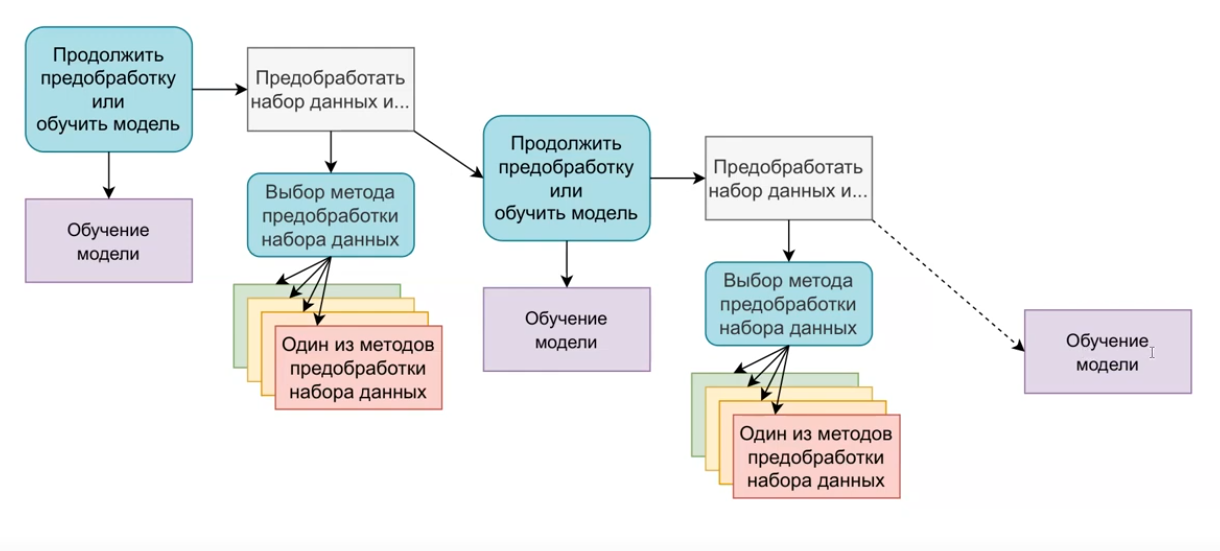
\includegraphics[scale=0.3]{images/rectree}
	\caption{Рекурсивная древовидная конфигурация.}
\end{figure}

Каждый раз спрашиваем себя обучить модель или предобработать
данные (выбрать один из методов предобработки).

\subsection*{Ациклическая конфигурация}

Херачим пути линейными конфигурациями, в конце обучаем
модели и ансамблируем.

\subsection*{RL для бедных}

Многорукими бандитами можно выбирать алгоритм, выполняя в
каждой ручке подбор гиперпараметров.